\section{Numerical solutions in the low frequency limit}
In this section we numerically solve the linear stability problem.  
We relax the thin-disk assumption, using the full, non-Keplerian
expressions of $\rho$, $\Omega$ and $\kappa$, so that we may consider
vertical domains up to $z\sim r$. However, we retain the low-frequency
approximation $|\sigma^2|\ll\kappa^2$ to obtain a linear eigenvalue
problem, which limits us to consider large radial wavenumbers
$k_x$. We will relax this in the next section when considering
moderate values of $k_x$. % This level of approximation lies in between
% the full problem Eq. \ref{iso_ode}, solved by \cite{mcnally14}, and
% the thin-disk limit Eq. \ref{iso_ode3}, solved by \cite{nelson13}.    


%We will solve different versions of the linearized equations depending
%on the disk properties, but in all cases we use 

\subsection{Vertically isothermal disks with isothermal
  perturbations}\label{vertiso_pertiso} 
We first validate the low-frequency approximation by re-producing
results from \cite{mcnally14} who solved the full problem for
vertically isothermal disks ($\Gamma=1$) subject to isothermal
perturbations ($\gamma=1$). The parameters are $q=-1$,
$p=-1.5$, $\epsilon=0.1$ and $k_x = 200\pi/r$ (or $\hat{k} = 20\pi$),
with solid vertical boundaries. 

For this problem we solve Eq. \ref{iso_ode}, with $D$ replaced by
$\kappa^2$, using a pseudo-spectral
method by expanding $W$ in Chebyshev polynomials $T_l$ up to $l=512$
and discretizing the equation on a grid with
$\zmax=10\epsilon r$. This procedure converts the linear problem
to a standard matrix eigenvalue problem.   

Fig. \ref{lowfreq_eigen} shows the eigenvalues $\sigma = \omega +
\ii\nu$. This plot is effectively identical to that in
\cite{mcnally14}. The fundamental VSI mode, with one node in $W$, has
the smallest $|\sigma|$ and is shown in Fig. \ref{lowfreq_eigenfunc}.  
The expected growth rate from Eq. \ref{simple_growth} with 
$L=1$ is  
\begin{align*}
  \nu = 0.2606\epsilon\Omega_k,
\end{align*}
as obtained numerically. This agreement is surpsingly good, given that
Eq. \ref{simple_growth} assumes the thin-disk approximation and
imposes a different boundary condition to that in the numerical
calculation. The eigenfunction $W$ is qualitatively proportional to
$z$, as expected for the fundamental mode according to explicit
solutions discussed in \S\ref{iso_poly}.    

\begin{figure}
  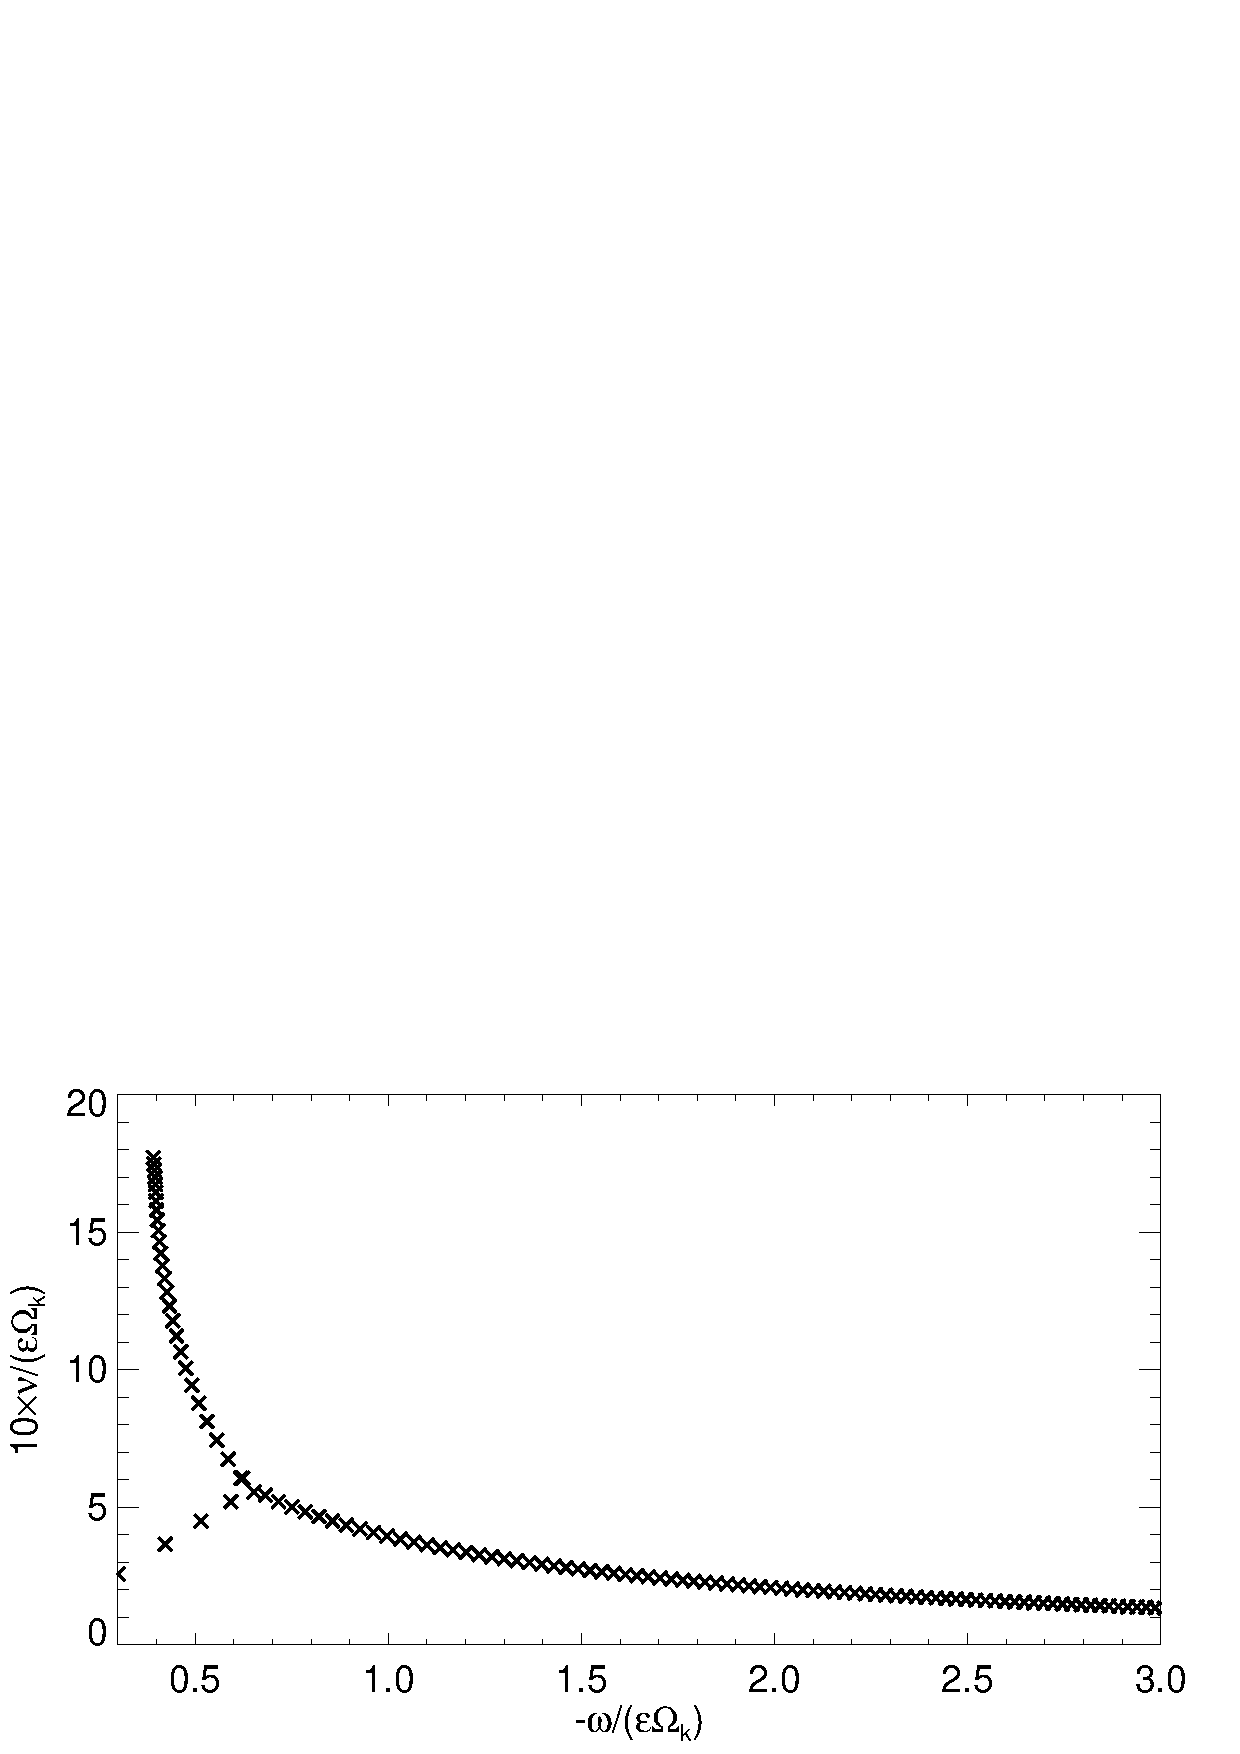
\includegraphics[width=\linewidth]{figures/eigenvalues_iso}
  \caption{Eigenvalues in the low-frequency approximation for the
    vertical shear instability in a vertically isothermal disk evolved
    isothermally ($\gamma=\Gamma=1$). The disk parameters are $q=-1$,
    $p=-1.5$ and $\epsilon=0.1$, while the perturbation radial
    wavenumber is $k_x=200\pi/r$. This is the set up considered in
    \cite{mcnally14}. \label{lowfreq_eigen}
  }
\end{figure}

\begin{figure}
  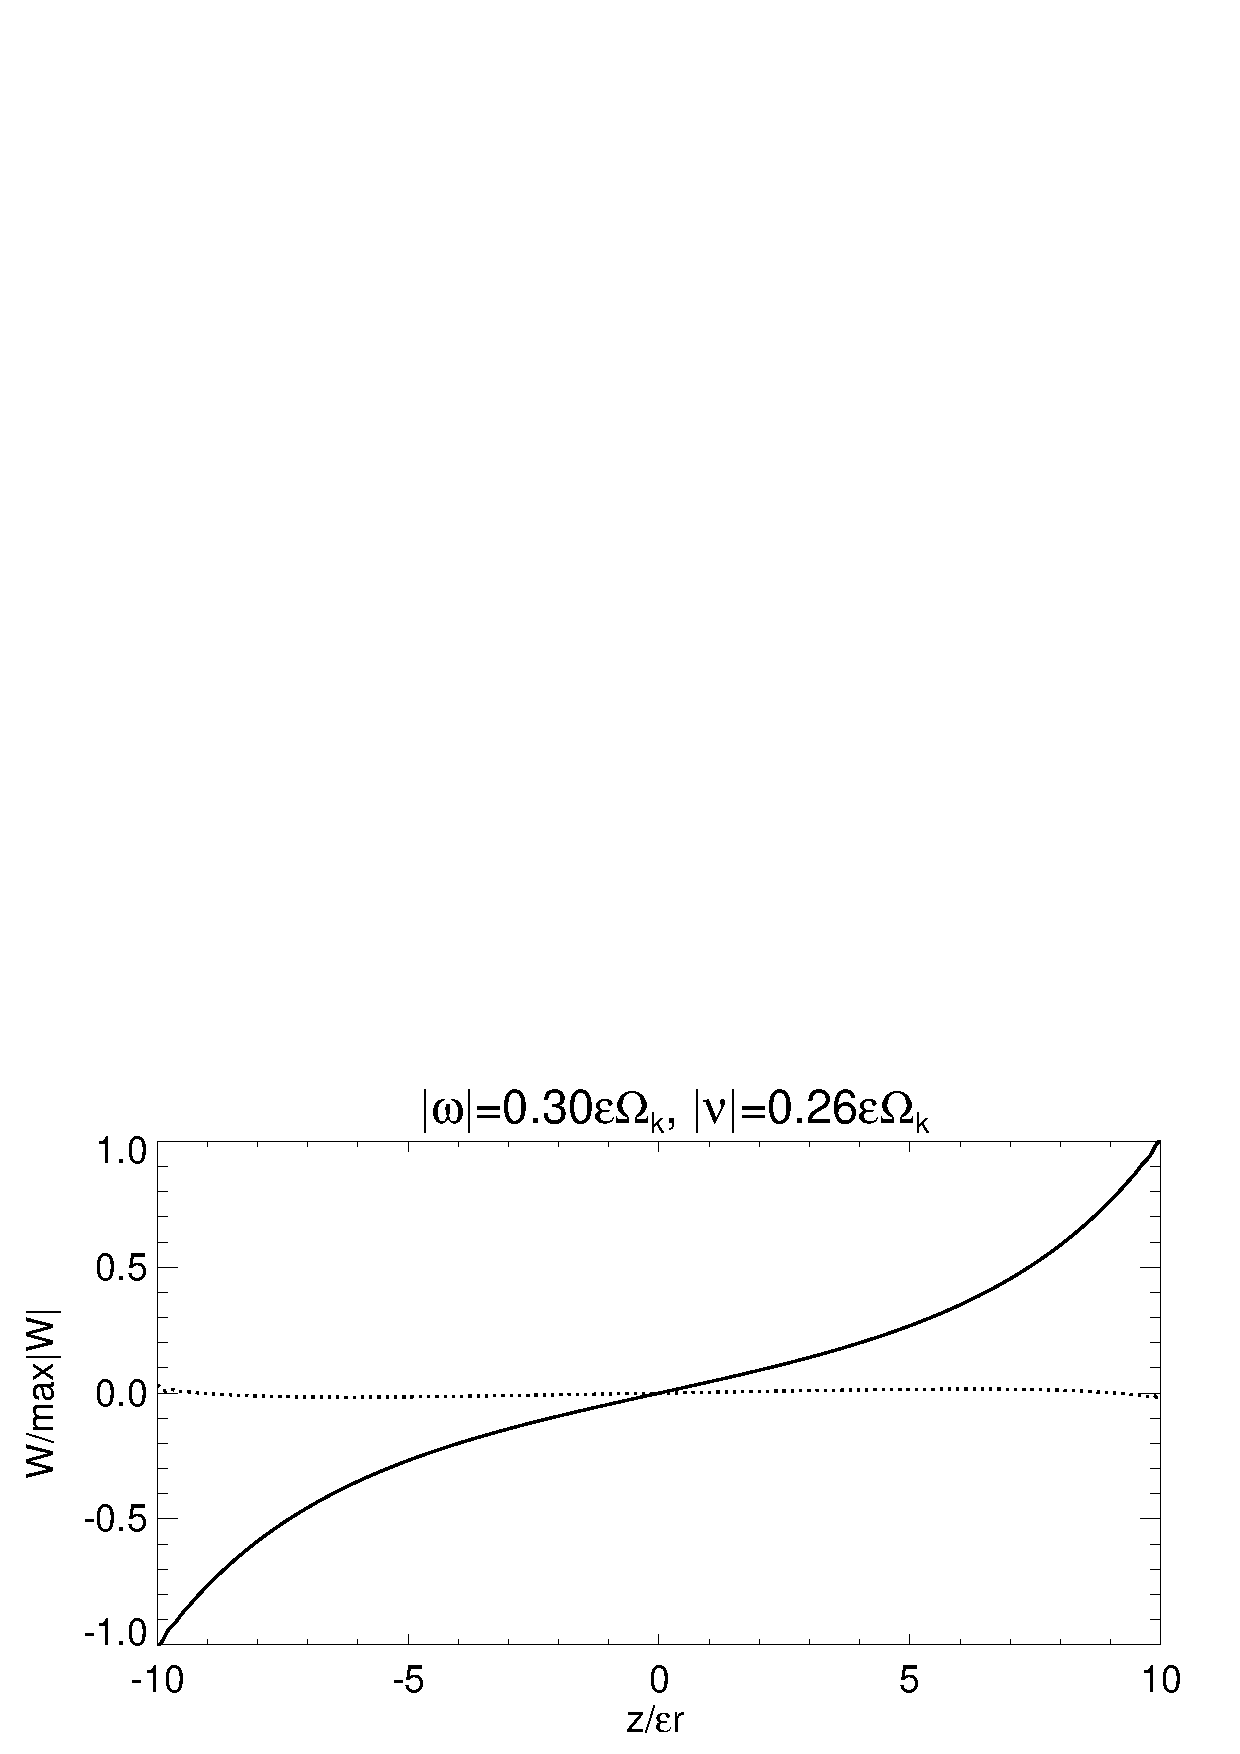
\includegraphics[width=\linewidth]{figures/eigenvector_iso}
  \caption{Eigenfunction of the fundamental VSI,
    corresponding to the bottom-left eigenvalue displayed in
    Fig. \ref{lowfreq_eigen} (smallest $|\sigma|$). The
    solid and dashed lines are $\real W$ and $\imag W$, respectively. 
    \label{lowfreq_eigenfunc}
  }
\end{figure}

\subsection{Stabilization of the VSI by a positive vertical entropy
  gradient}
We demonstrate the (strong) stabilizing effect of a  
positive vertical entropy gradient. We solve the more general form of
the linear problem, Eq. \ref{ode_w}---\ref{ode_Q}, again with the
replacement $D\to\kappa^2$. We consider an effectively vertically
isothermal disk by setting $\Gamma=1.011$ with adiabatic index
$\gamma=2$. We also set $\beta=10^9$ so the cooling term is
effectively switched off. Other disk and perturbation parameters are
the same as in \S\ref{vertiso_pertiso}. 

We use the same pseudo-spectral method as before. Here we set
$\zmax = 2\epsilon r$ and impose a free surface. This boundary
condition was found to be most convenient for numerical
implementation. Since we expect the perturbations to decay rapidly
away from the midplane (see \S\ref{analytic_adia}), we do not expect 
boundary conditions to play an important role, provided that $\zmax$ is
sufficiently large. 

Fig. \ref{lowfreq_eigen_adia} show the eigenvalues for this
problem. The growth rates are about an order of magnitude smaller than
the previous case. The fundamental VSI mode is that with
$\mathrm{max}|\nu|$. Its expected and numerically-calculated growth
rates compares well, with 
\begin{align*}
  \nu = 0.03751 \epsilon \Omega_k &\quad \text{(from
    Eq. \ref{gam2_growth_rate})},\\
  \nu = 0.03682 \epsilon \Omega_k &\quad \text{(numerical)}.
\end{align*}
The fundamental mode is plotted in Fig. \ref{lowfreq_eigenfunc_adia},
and clearly show that perturbations are rapidly stabilized away from
the midplane. For the adopted disk and perturbation parameters 
($|q|=1$ and $\hat{k} = 20\pi$), Eq. \ref{gam2_alpha} gives $\real{\alpha}\simeq - 43.8$,
corresponding to a characteristic decay lengthscale of $\simeq
0.15\epsilon r$, which is consistent with that observed in 
Fig. \ref{lowfreq_eigenfunc_adia}. 

\begin{figure}
  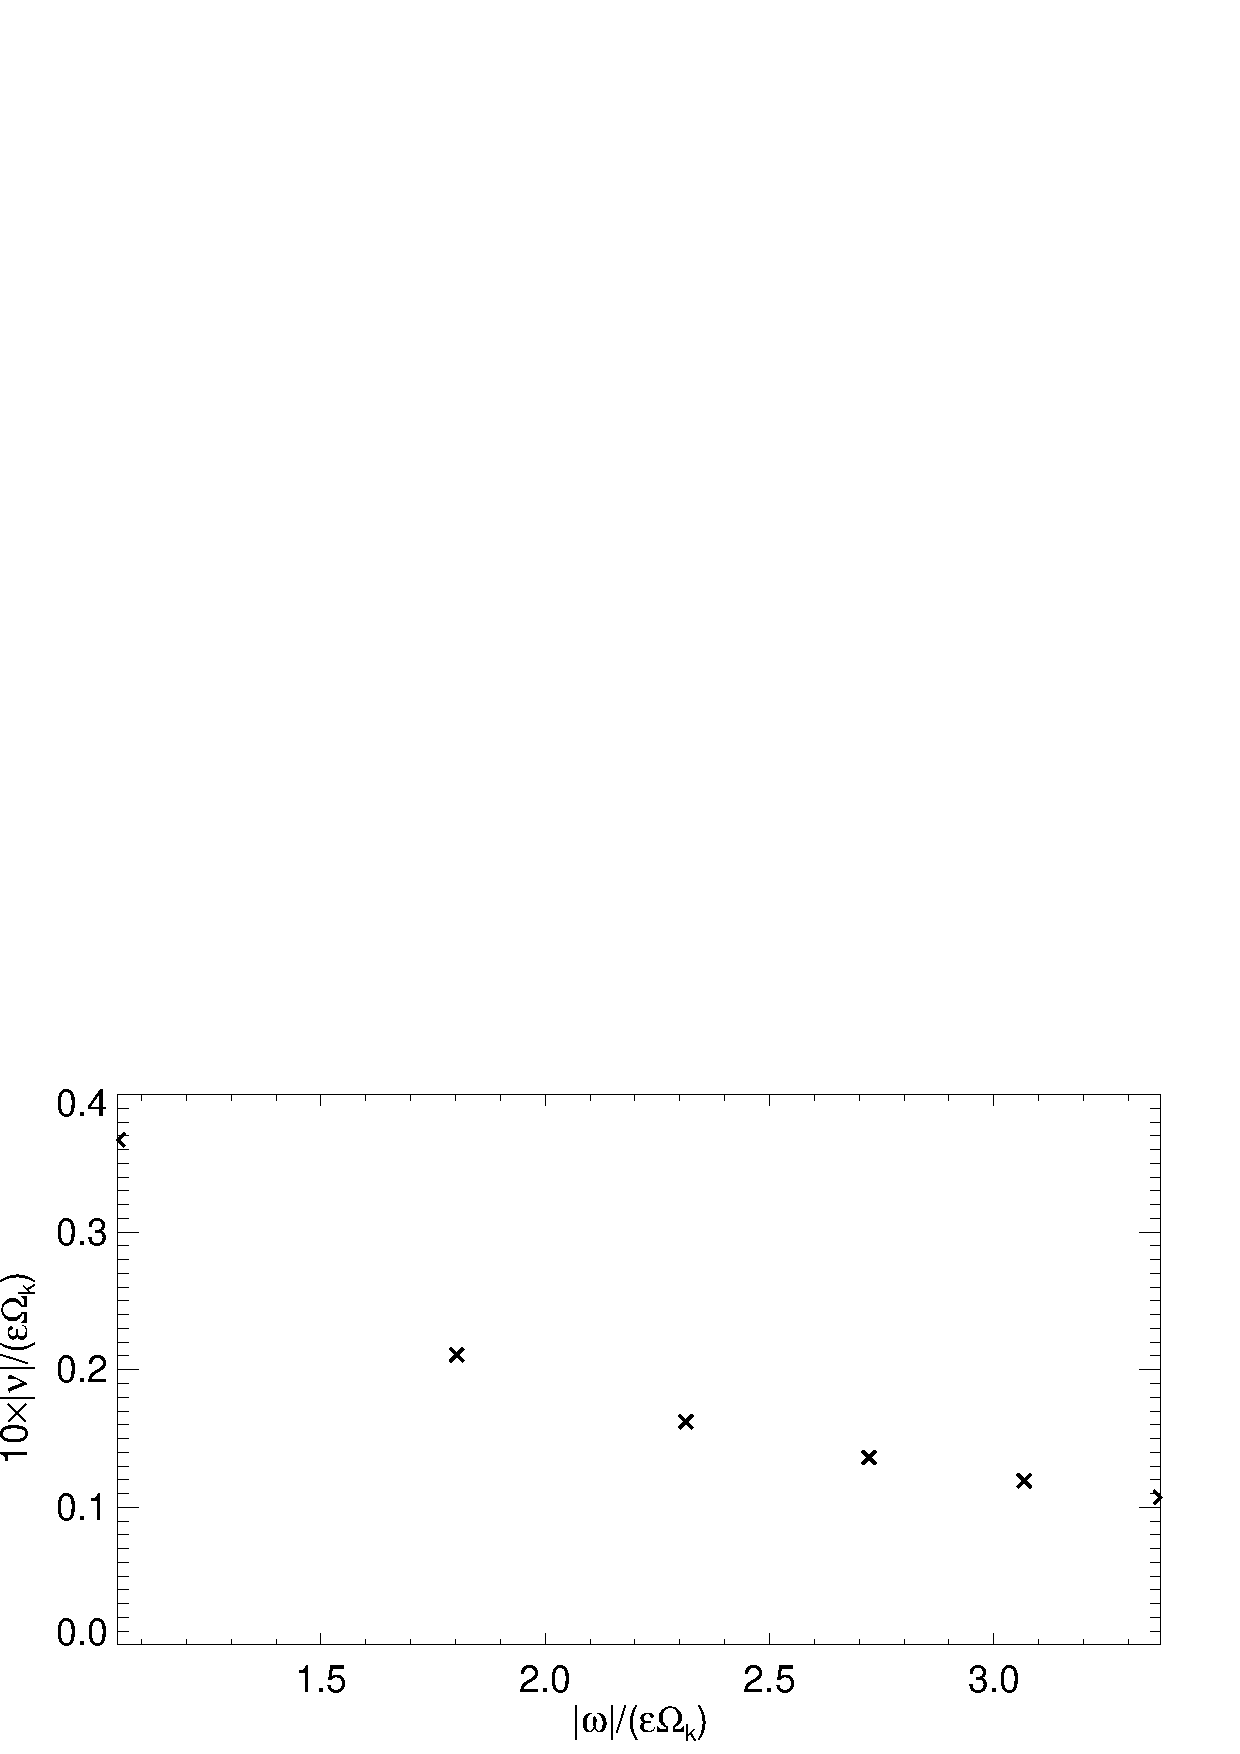
\includegraphics[width=\linewidth]{figures/eigenvalues_adia}
  \caption{Eigenvalues in the low-frequency approximation for the
    vertical shear instability in a nearly-vertically isothermal disk
    ($\Gamma=1.011$) evolved adiabatically with $\gamma=2$ and
    $\beta=10^9$. The disk
    parameters are $q=-1$, 
    $p=-1.5$ and $\epsilon=0.1$, while the perturbation radial
    wavenumber is $k_x=200\pi/r$. \label{lowfreq_eigen_adia}
  }
\end{figure}
  

\begin{figure}
  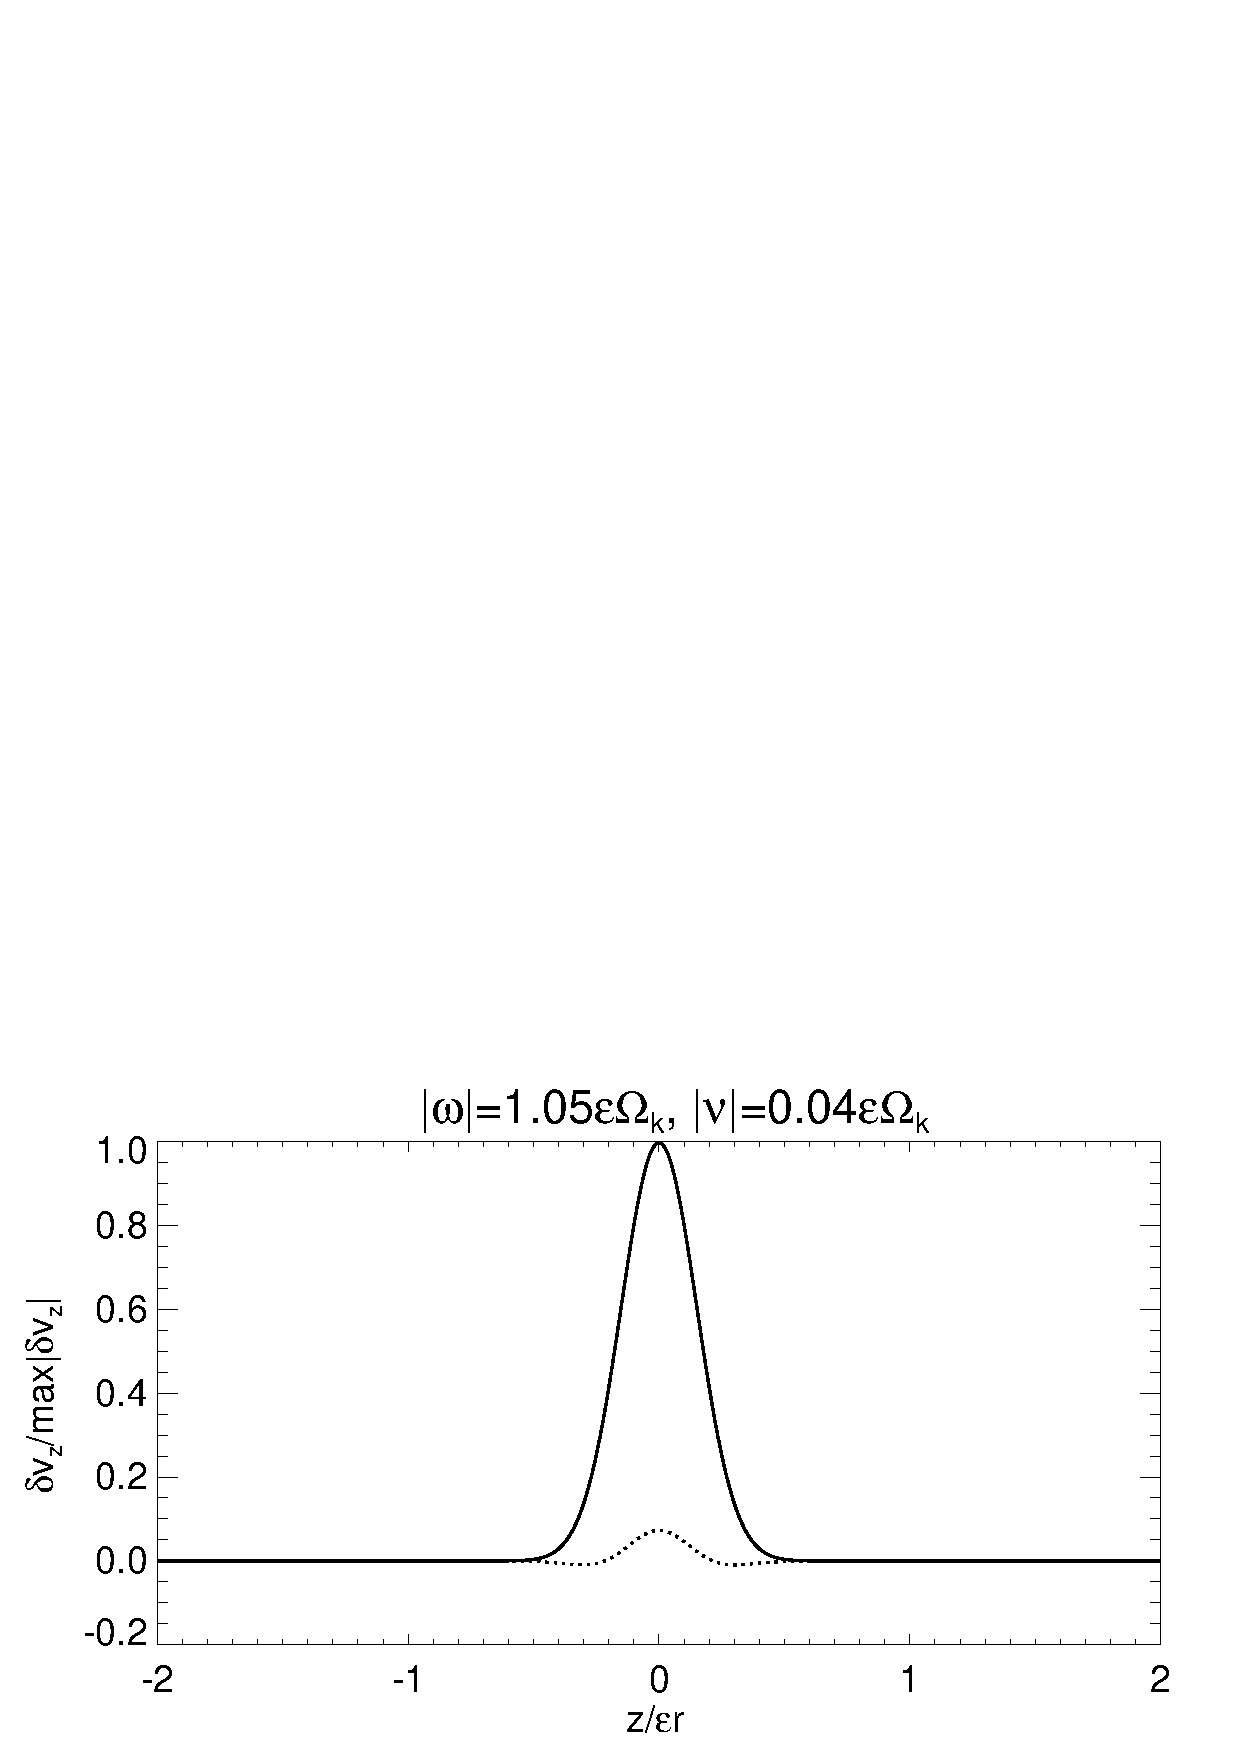
\includegraphics[width=\linewidth]{figures/eigenvectorvz_adia}
  \caption{Fundamental VSI mode in a nearly-vertically
    isothermal disk ($\Gamma=1.011$) evolved adiabatically
    ($\gamma=2$, $\beta=10^9$). This eigenfunction 
    corresponds to the top-left eigenvalue displayed in 
    Fig. \ref{lowfreq_eigen_adia} (largest $|\nu|$).  
    The solid and dashed lines are $\real \delta v_z$ and $\imag
    \delta v_z$, respectively.  
    \label{lowfreq_eigenfunc_adia}
  }
\end{figure}

\subsection{Effect of cooling} 